\documentclass[a4paper, titlepage]{article}
\usepackage[T1]{fontenc}
\usepackage[utf8]{inputenc}
\usepackage[english]{babel}
\usepackage{siunitx}
\usepackage{graphicx}
\usepackage{amsmath}
\usepackage{amsmath}
\usepackage{amssymb}
\usepackage{caption}
\usepackage{refstyle}
\usepackage{circuitikz}
\usepackage{subfig}
\usepackage{gensymb}
\usepackage{adjustbox}
\usepackage{latexsym}
\usepackage{float}
\usepackage{hyperref}
\usepackage[a4paper,top=2.5cm,bottom=2.5cm,left=2.5cm,right=2.5cm]{geometry}
%\usepackage[left=3cm, right=3cm, top=3cm]{geometry}

\usepackage{fancyhdr}
\pagestyle{fancy}
\lhead{}
\fancyhead[L]{\leftmark}
\lfoot{}
\cfoot{}
\rfoot{}
\rhead{\thepage}
%
\usepackage{rotating}
\usepackage{booktabs, longtable,afterpage}
\usepackage{rotating}
\usepackage{makecell}
\graphicspath{ {images/} }
\begin{document}
\begin{titlepage}
	\centering
	
\includegraphics[width=0.40\textwidth]{Politecnico_di_Torino_-_Logo}\par\vspace{1cm}
	\vspace{1cm}
	{\huge\bfseries Integrated Systems Architecture\par}
	\vspace{1cm}
	{\scshape\Large Lab 1: design and implementation of a digital filter \par}
	\vspace{2,5cm}
	{\Large\itshape Group 30:\\Chisciotti Laura 274728\\Fusto Federico 279925 \\Goti Gianluca 269825\par}
	\vspace{2,5cm}
		{\Large\bfseries Github repository: \url{https://github.com/Gotg3/ISA_Lab1.git}\par}
	\vfill

	\vfill
	{\Large A.Y. 20-21}
\end{titlepage}
\newpage
\tableofcontents
\newpage


\section{Introduction}
In this lab, the goal is to design a digital filter with a cut-off frequency of 2 kHz and a sampling frequency of 10 kHz.\\The schematic structure of the digital filter is shown in Figure \ref{fig:filt_arch} and it is possible to observe that the filter must include an active-low RESET signal, a validation signal VIN for the inputs and another signal, VOUT, for the outputs, moreover its parallelism is equal to $n_{b}$ bits.
 \begin{figure} [h]
\centering
	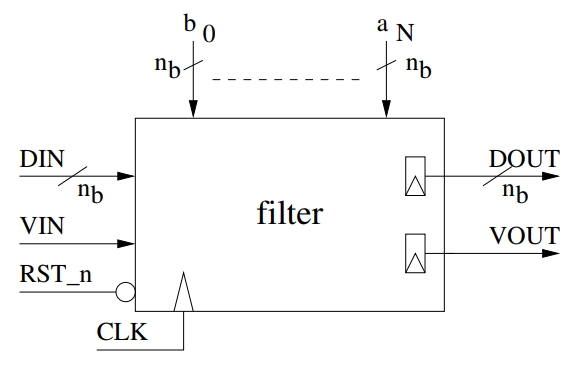
\includegraphics[scale=0.6]{filt_arch.PNG}
	\caption{Schematic filter architecture}
	\label{fig:filt_arch}
\end{figure}
\newline The first part concerns the design of the filter with Matlab and C implementation, the latter being the reference for the comparisons.\\The second part examines the outputs of the VHDL implementation that will be compared with the references. Once proved, the filter will be synthesized with Synopsys Design Compiler, thus it will be placed and routed with Cadance SOC Innovus.\\
Finally, several advanced architecture techniques will be applied in order to maximize the performance of the filter.\\
It is important to take into account that the filter implementation has been performed without the design of a Finite State Machine that generates all the control signals for the datapath since in this specific case it comes down to a sequence of registers and for this reason its usage results to be overengineered.\\
Thus, controls have been generated by properly delaying the enable signal VIN.
 
\section{Reference model development}
\subsection{Filter design and coefficient quantization using Matlab/Octave}
First of all, the type of filter, order and parallelism have been determined using an algorithm based on the group number and surnames of the components. Being the group number equal to 30, the filter is an IIR type.\\
%%%%%%%%%%
%VERSIONE NUOVA
%%%%%%%%%%%
Then the order of the filter \textbf{N} and the number of bits \textbf{n$_{b}$} to represent the coefficients have been computed from the first two surnames of the teammates listed in alphabetical order. \\The algorithm used to determine these two parameters is the following:
\begin{equation}
    N=2^{p}\cdot[(x\; mod\; 2)+1]+6\cdot p
\end{equation}
\begin{equation}
    n_{b}= (y\; mod\; 7) + 8
\end{equation}
where \textit{x} and \textit{y} have been assumed as the number of characters of the first two surnames members. Therefore, since the first two surnames are Chisciotti and Fusto, the input parameters of the algorithm have been found to correspond to $x=10$ and $y=5$, thus the resulting parameters are:
\begin{itemize}
    \item [$-$] $N=1$
    \item [$-$] $n_{b}=13$
\end{itemize}

%%%%%%%%%%%%%
%VERSIONE VECCHIA
%%%%%%%%%%%
%Then the order of the filter \textbf{N} and the number of bits to represent the coefficients \textbf{n$_{b}$} have been computed from the first two surnames of the teammates listed in alphabetical order, obtaining:
%\begin{itemize}
   % \item [$-$] $N=1$
   % \item [$-$] $n_{b}=13$
%\end{itemize}
%The parameters had to be set following this algorithm and assuming $x$ and $y$ as the number of characters of the first two surnames members:
%\begin{equation}
%    N=2^{p}\cdot[(x\; mod\; 2)+1]+6\cdot p
%\end{equation}
%\begin{equation}
%    n_{b}= (y\; mod\; 7) + 8
%\end{equation}
%Since the first two surnames are Chisciotti and Fusto, therefore the input parameters of the algorithm have been found to correspond to $x=10$ and $y=5$, thus the resulting parameters are:
%\begin{itemize}
%    \item [$-$] $N=1$
%    \item [$-$] $n_{b}=13$
%\end{itemize}
\newpage

\subsection{Testing the filter and fixed point implementation}
At this point, the filter has been tested in Matlab using a signal consisting of two sinusoidal waves ($x=\dfrac{x_1+x_2}{2}$) at two different frequencies one of which in band (f$_1$ =500 Hz) and one out of band (f$_2$ =4,5 kHz). These signals are reported in Figure \ref{fig:sine_wave} and the resulting signal, represented in green, as well.
 \begin{figure} [h]
\centering
	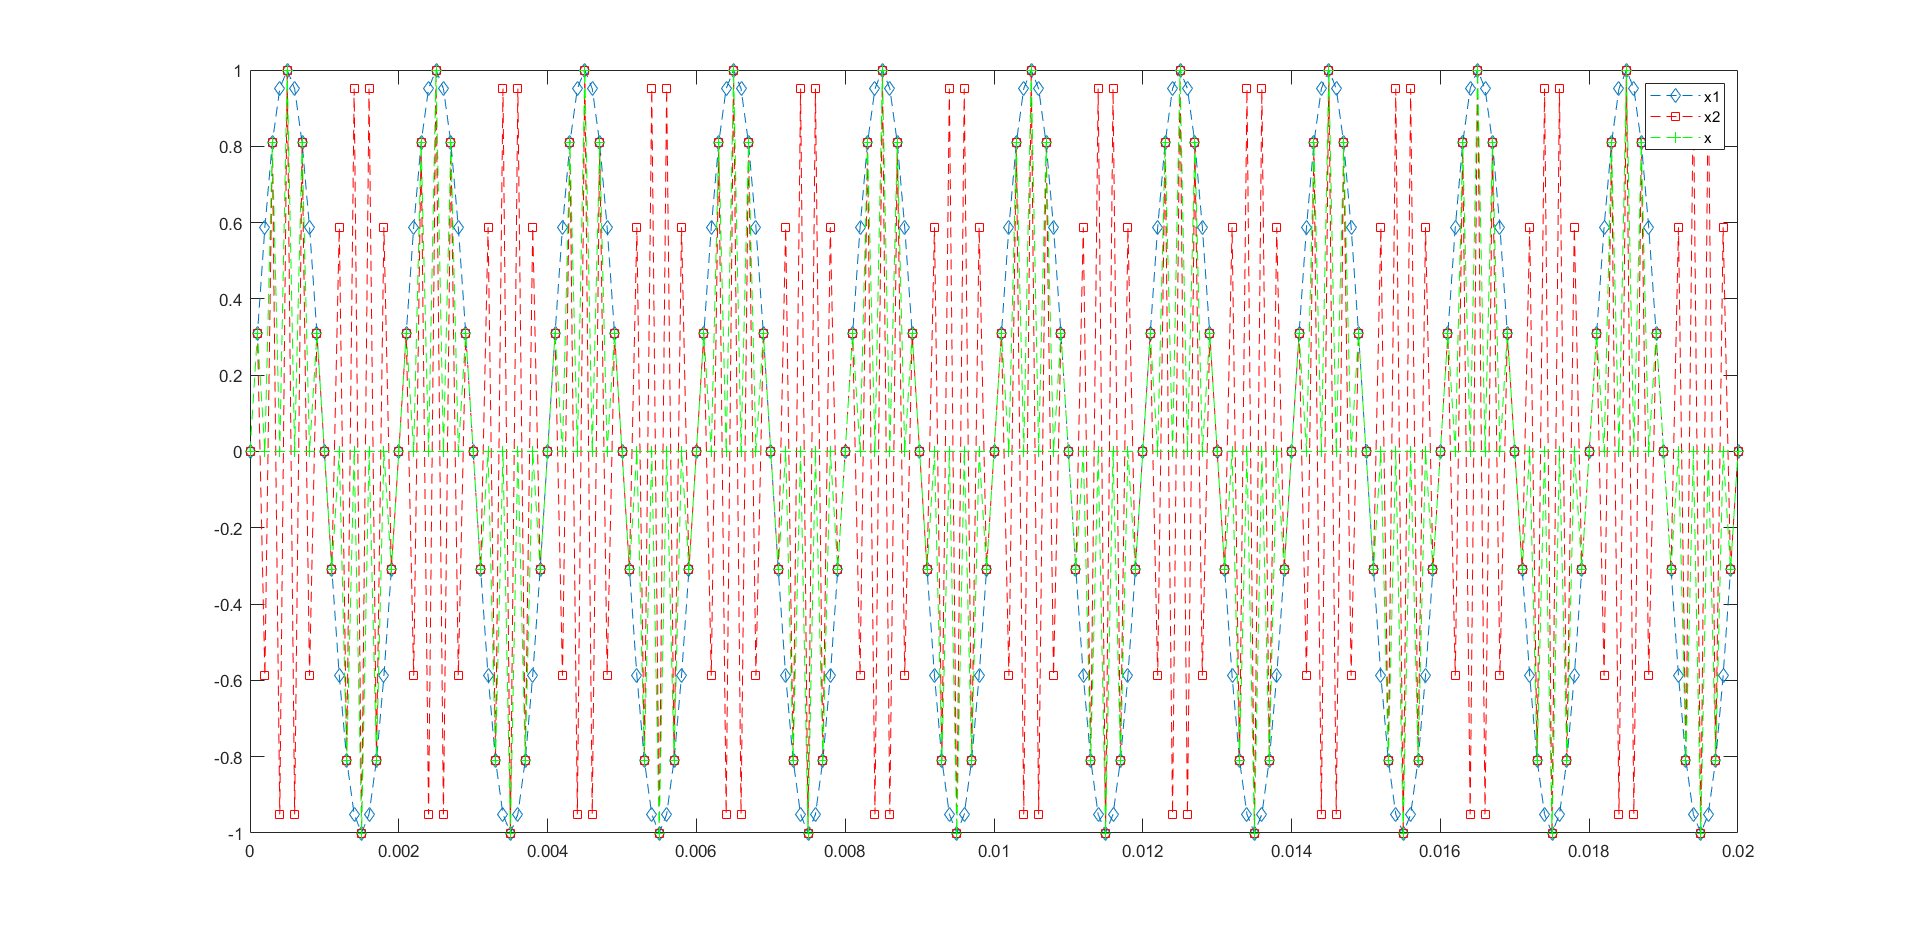
\includegraphics[scale=0.25]{inputs.png}
	\caption{Sinusoidal signal}
	\label{fig:sine_wave}
\end{figure}
\noindent 
In Figure \ref{fig:x_y_filter} the input and the output signals of the filter have been reported. From the plot is possible to observe that the output signal has a period similar to the in band signal, since the filter has attenuated all the components higher than the cut off frequency. Furthermore, the amplitude has been reduced, but this is reasonable because this is a passive filter.
 \begin{figure} [h]
\centering
	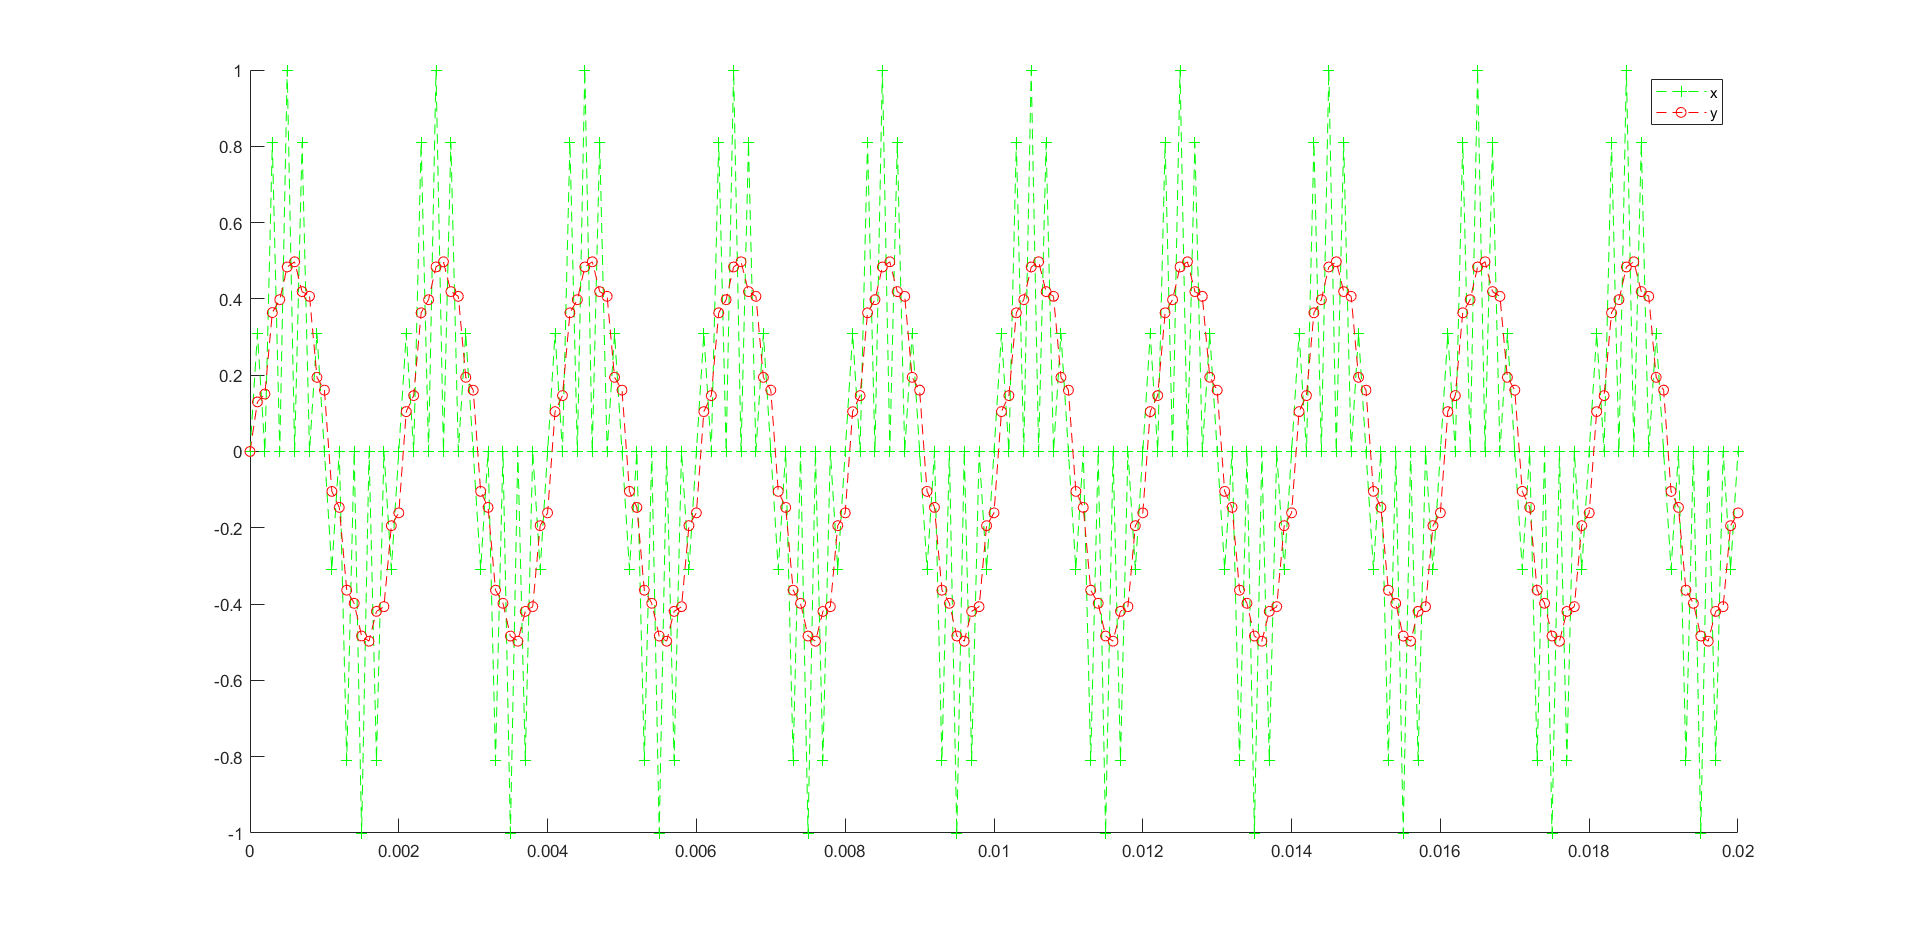
\includegraphics[scale=0.25]{y_x_filter.png}
	\caption{Input and output of the filter}
	\label{fig:x_y_filter}
\end{figure}
\noindent
\newline
Then, a fixed point implementation of the IIR filter \textbf{direct form II} has been implemented in C-language and the corresponding DFG is reported in Figure \ref{fig:IIR filter scheme}.
\begin{figure} [h]
\centering
	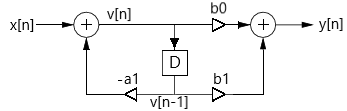
\includegraphics[scale=0.9]{IIR_filter_scheme.png}
	\caption{Direct form II scheme for IIR filter}
	\label{fig:IIR filter scheme}
\end{figure}
\newline
The discrete-time equations about this type of IIR filter are respectively:
\begin{equation}
\label{eq:IIR eq}
    y[n]=b_0\cdot v[n]+b_1\cdot v[n-1]
\end{equation}
With:
\begin{equation}
\label{eq:IIR eq v[n]}
    v[n]=x[n]-a_1\cdot v[n-1]
\end{equation}
Where b$_0$ and b$_1$ are the coefficients of the moving average part and a$_1$ is the coefficients of the auto-regressive part.\\
From Matlab, coefficients b$_0$, b$_1$ and a$_1$ have been calculated setting N=1 and n$_b$=13, assuming the following $n_b$ bits real values:
\begin{itemize}
    \item[--] b$_0$= 1723
    \item[--] b$_1$= 1723
    \item[--] a$_1$= -649
\end{itemize}
 Then, these coefficients have been inserted in the C implementation of the IIR filter from which the result \textit{y} of the fixed point implementation has been obtained.\\ 
At this point, the Total Harmonic Distortion (THD) of the output has been calculated using the \textit{thd} function in Matlab. As reference, the THD with the Matlab results have been computed (Fig.\ref{fig:thd_matlab}) and this is equal to -79,68 dB. Since the task was to implement the filter as an hardware architecture, also the "C" results have been used to estimate the corresponding THD (Fig.\ref{fig:thd_c}).\\
From the specifications, the maximum value required is -30dB while the filter's value is -69,15 dB, so the required constraint is met.\\
As one can observe, in the "C" fixed point implementation, the higher order harmonics are less attenuated than the Matlab implementation, on avarage of a decreasing of 10 dB or so.

 \begin{figure} [h]
\centering
	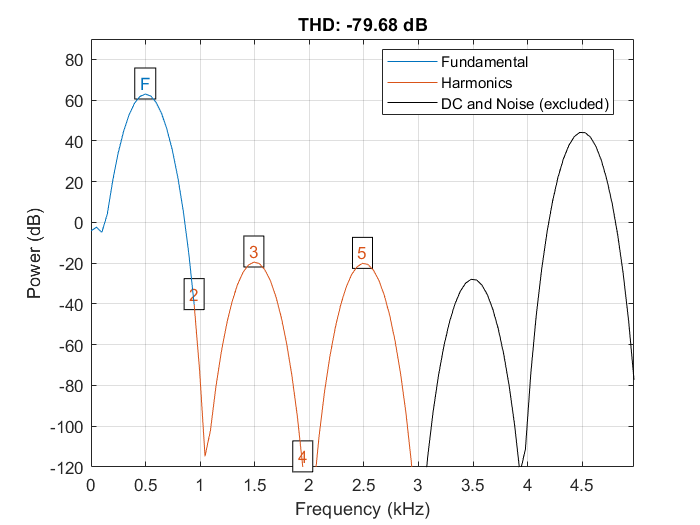
\includegraphics[scale=0.6]{THD_matlab.png}
	\caption{THD with results from Matlab}
	\label{fig:thd_matlab}
\end{figure}
\newpage
 \begin{figure} [h]
\centering
	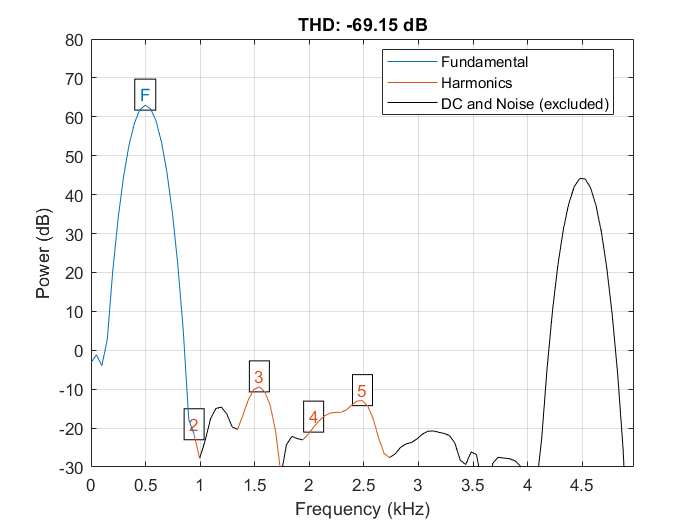
\includegraphics[scale=0.6]{THD_C.png}
	\caption{THD with results from C implementation}
	\label{fig:thd_c}
\end{figure}
\noindent
In Figure \ref{fig:freq_res_matlab} the transfer functions of the "real" filter is compared with the "quantized" one, as one can see the behaviour is practically the same.

 \begin{figure} [h]
\centering
	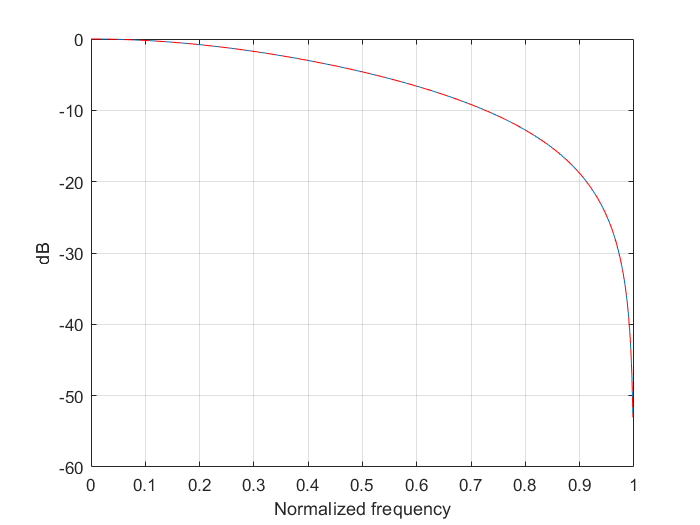
\includegraphics[scale=0.6]{filtresponse_nb13.png}
	\caption{"Real" filter vs "quantized" filter}
	\label{fig:freq_res_matlab}
\end{figure}
\newpage
\section{VLSI implementation}
\noindent
At this point the VHDL architecture of the filter has been implemented.\\The behaviour of the input and output signals is that the signal DIN for the samples has to be sampled when the validation signal VIN is asserted, while the validation signal VOUT has to be asserted when DOUT is ready.
\newline
Thus, starting from $n_{b}=13$, the parallelism has been increased to 14 bit to take into account the bit-growth during the 2's complement operations. Since the operations are represented in a fractional bit format, only additions are responsible for overflow problems which leads to the "wrap around" phenomena.
%responsible for smth
\newline
It has been proved that \textbf{1 additional internal bit} was sufficient to give the possibility to the inner amounts to grow during the various addition operations. This operation leads to have 14 internal bits.
\newline
This problem is particularly severe when one is working with 2's complement, since when an overflow occurs the represented value will result into a negative number. 
\newline
The hardware description has been chosen to be behavioural, to have an identical structure as the C-implementation.\\
This latter in practice does not care about overflows, since all computations are performed on \textit{int} variables. 
\\ %DOC
Because of this, some changes have been carried out to the C implementation in order to have the same behaviour in terms of bit representation (13 bits) and internal bit-growth (14 bits).
%At the same time, some changes have been carried out to the latter in order to have the same behaviour in terms of internal bit-growth.  
In the C filter, after all the multiplications the Chopping method has been used to limit the bit-growth, keeping the results on 14 bits. For this reason also the hardware implementation has been designed in the proper way to take into account this difference. 
\\Furthermore in the architecture two sets of registers have been used to sample input and output values, thus there will be an additional latency of 2 clock cycles.


\subsection{Starting architecture implementation}
In Figure \ref{fig:filter_base_version} is reported the datapath of the hardware implementation of the filter.
 
  \begin{figure} [h]
\centering
	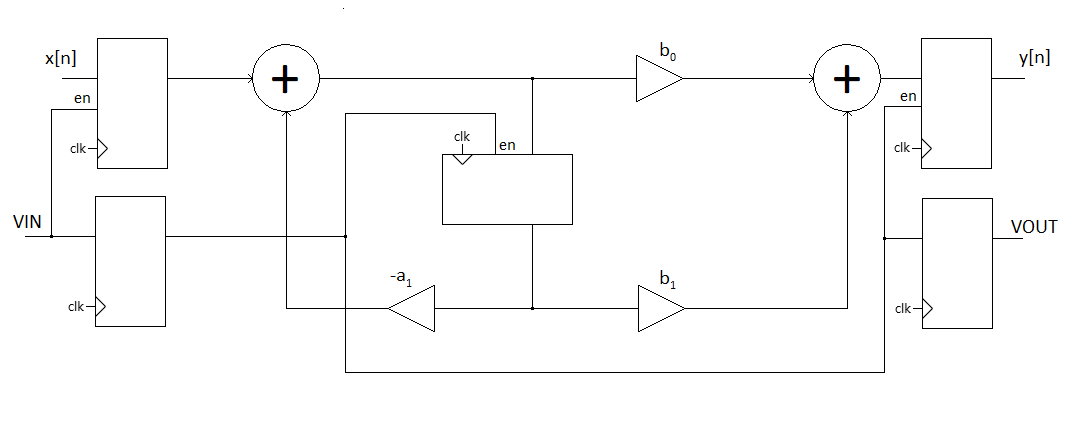
\includegraphics[scale=0.4]{filter_base_version.png}
	\caption{Datapath direct form II IIR filter}
	\label{fig:filter_base_version}
\end{figure}
\noindent In this architecture the VIN signal is used as an enable for the sampling registers, moreover when VIN=0 the input is not sampled and the previous one is kept at the output. 
 \newline
 Given that, these latter can be seen as pipeline registers, it has been necessary to properly delay VIN, as shown in the datapath.\\
 The VOUT signal has been generated delaying VIN to be synchronised with the output samples. It is important to notice that the input and output register used for this purpose do not need an enable signal since VIN and VOUT have to be sampled and generated in any case. 
 \newline
 Similarly to the previous cases, the internal register keeps the old data when the internal signal VIN is 0.
 \newpage
 \subsection{Simulation}
 
 
The first two simulations reported in Figure \ref{fig:start_sim} and Figure \ref{fig:end_sim} show respectively the start and the end of the computation, with VIN asserted to sample DIN and VOUT asserted when DOUT is ready. 

\begin{figure} [h]
\centering
	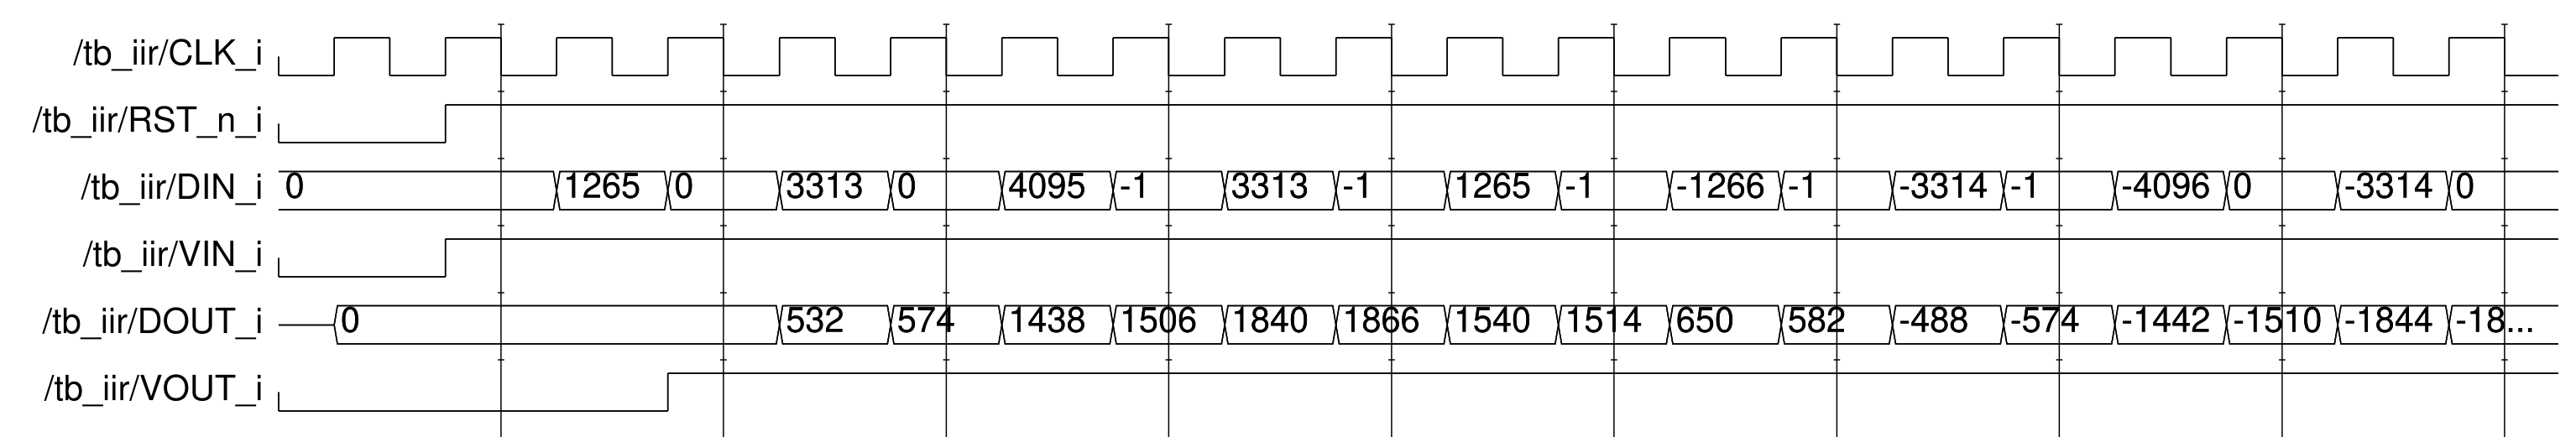
\includegraphics[scale=0.55]{start_sim.png}
	\caption{Filter simulation "start"}
	\label{fig:start_sim}
\end{figure} 

 \begin{figure} [h]
\centering
	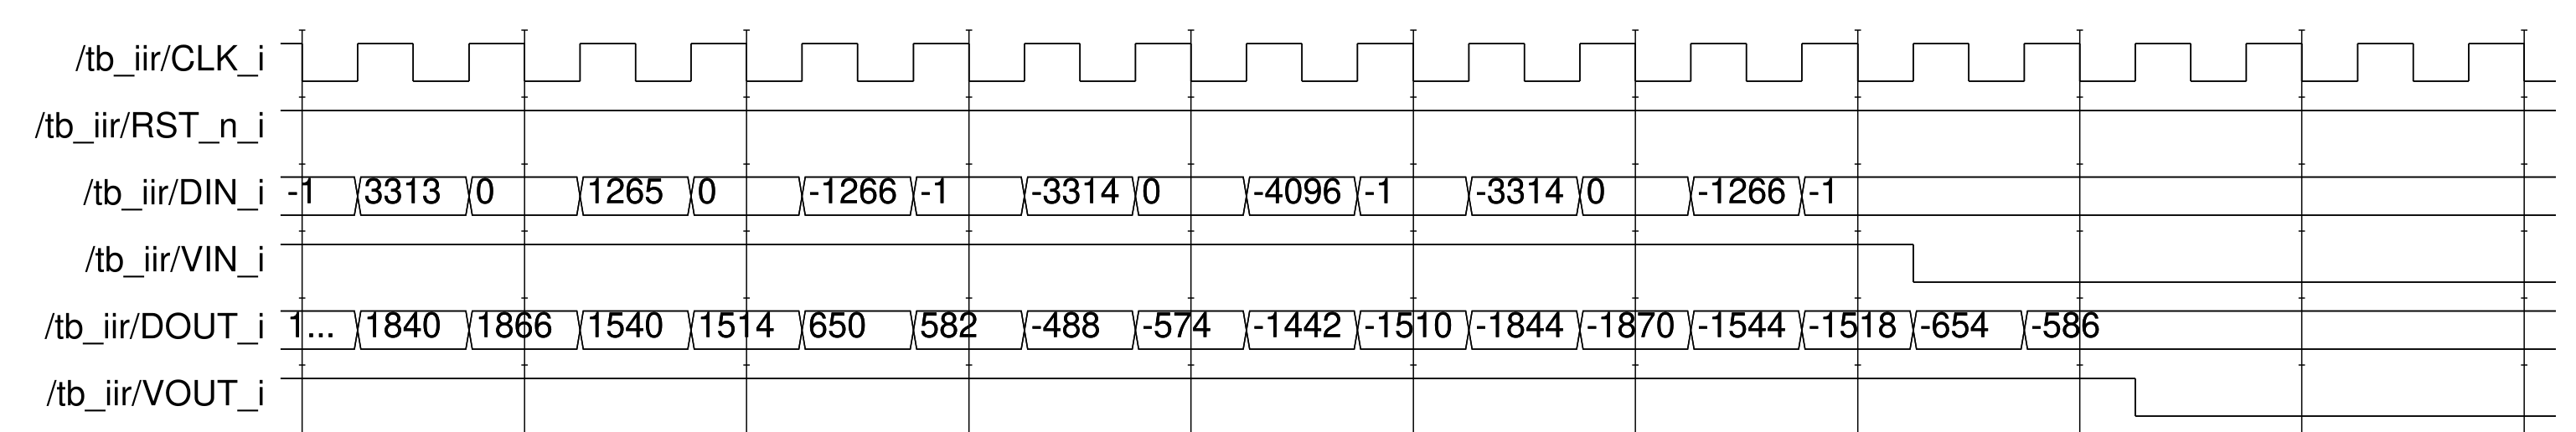
\includegraphics[scale=0.55]{end_sim.png}
	\caption{Filter simulation "end"}
	\label{fig:end_sim}
\end{figure} 
    
\noindent In order to verify the correct behaviour of the architecture, a testbench where DIN has been properly driven has been used.
%nuova versione
In Figure \ref{fig:vin_sim} it is possible to observe how the architecture reacts when VIN is 0. One can notice that when this latter is low the internal computations stops and the output remains unchanged.
%In fact starting from when VIN in asserted and DIN=0 in sampled, then VIN goes down and accordingly the internal computation stops thus the output value remains unchanged.
  \begin{figure} [h]
\centering
	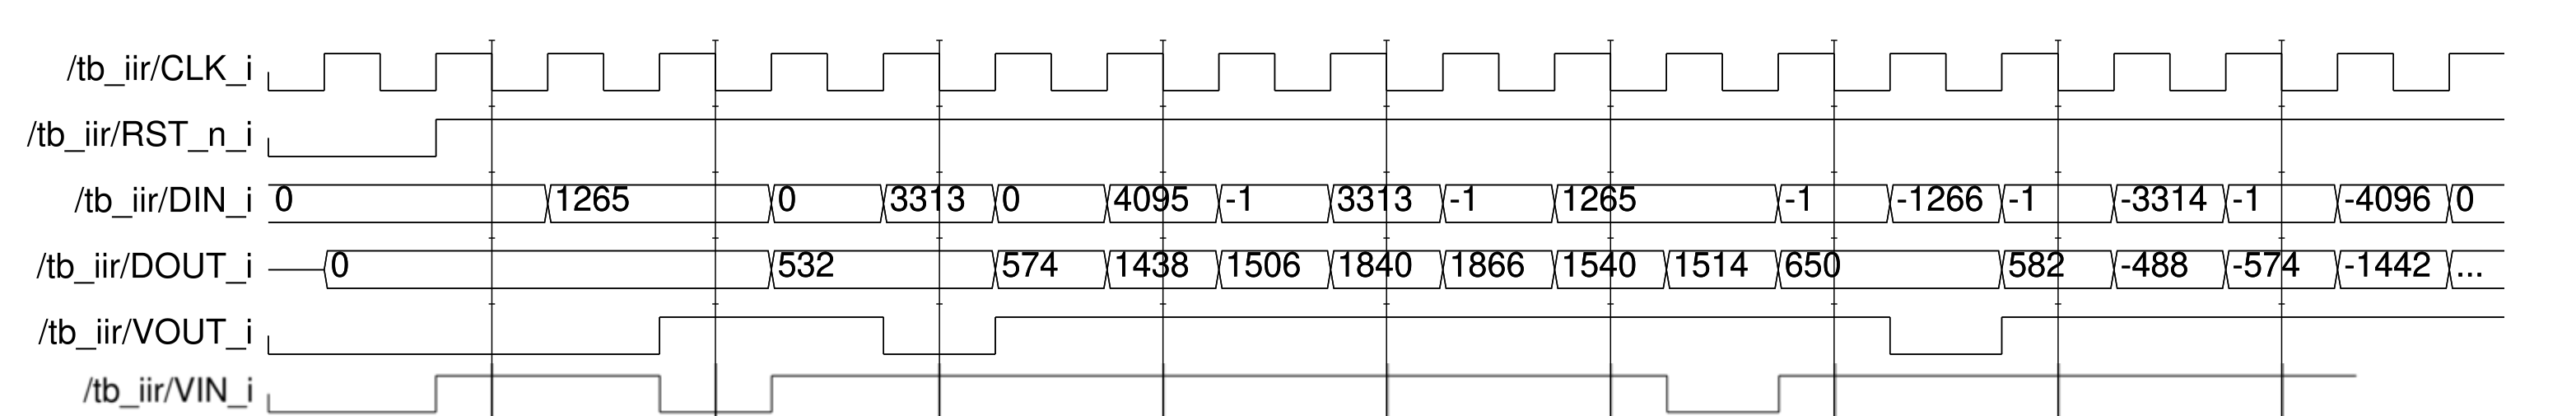
\includegraphics[scale=0.12]{image.png}
	\caption{Filter simulation with VIN variations}
	\label{fig:vin_sim}
\end{figure} 

\noindent Once the correct behaviour has been verified, the comparison of the results produced by the VHDL and C implementation has been computed.
Using a Matlab script the sum of the differences between the two output samples has been performed, all the values of the two implementations result to be identical.

\newpage
\subsection{Implementation}
\subsubsection{Logic synthesis}
After the implementation phase the design has been synthesized using Synopsys Design Compiler. The filter architecture has been elaborated and analysed, then constraints have been applied to proceed with the timing analysis.
\newline
The first step has focused to the research of the maximum clock frequency of the design $f_{M}$, to do that a clock signal named MY\_CLOCK has been created, with a period of $T_{min} \;[ns]$. Then, considering that the clock could be affected by jitter, an uncertainty of $0,07 \; ns$ has been applied. Next, an input and output delay has been applied, assuming that signals could arrive with some delay with respect to the clock signal. It has been assumed that both signals had the same maximum delay, equal to $0,5 \; ns$. These contributions have been considered in the overall timing analysis, simply by adding them to the computation once.
\newline
To perform all the correct analysis, a load for each output has been set and For the sake of simplicity a single reference buffer has been used, named BUF\_X4 and available in the provided library.
\newline
Then to find the minimum architecture clock period, initially a period of $0\; ns$ has been set in the first synthesis, obtaining the minimum period equal to $T_{min}=3\; ns$.  This value is the minimum achievable clock period  since the slack was zero (the difference between the timing required and the one achieved), thus the maximum achievable frequency of the design is $f_M \simeq 333,3 \;MHz$.
\newline 
Afterward, to find the area of the architecture, a new synthesis has been performed with the correct value of the clock period. 
From the area report it has been found that the total cell area is $A_{f_M}\simeq3045,97 \; \mu m ^2$. 
\newline 
The whole area isn't reported because the tool had only the information about the cells in the architecture, any information has been provided to estimate the area of the interconnections, in fact the Net Interconnection Area is undefined. Thus, to have a complete estimation of the area of the design, information about the interconnections is needed.
\newline
Then a new synthesis has been performed using a frequency equal to $\dfrac{f_M}{4}$ ($T_{min}= \;12 \;ns)$ in this case the total cell area is $A_{f_M/4}\simeq2501,46\; \mu m ^2$. It is possible to notice that the Total Cell Area is decreased and this could depend on the instance of different elements compared to the previous case.
%is decreased/increased : It's common to use passive present to describe something that has happened "on its own" with no person or definite subject causing it.
because probably  Synopsys has chosen slower components which are less demanding in terms of area. With a more detailed look to the report, one can notice that in the initial architecture with a frequency $f_M$ the Combinational Area and the Buf/inv Area are greater than the ones in the $\dfrac{f_M}{4}$ implementation. This is reasonable because if the design is faster, it needs faster blocks (i.e. more efficient and faster adders) and it also needs more buffers, to cut the long interconnections and to decrease the propagation delay along them.
\newline
All the data related to the areas are reported in Table \ref{tab:area base fm vs fm/4}.

\begin{longtable}{*6c}
\caption{Area $f_M$ vs Area $\dfrac{f_M}{4}$}
\label{tab:area base fm vs fm/4}\\
\toprule
Clock freq. & \thead{Combinational \;[$\mu m^2$]} & \thead{Buf/Inv\;[$\mu m^2$]} & \thead{Tot.\; Cell \;Area\;[$\mu m^2$]} \\
\midrule
\endfirsthead
Clock freq. & \thead{Combinational \;[$\mu m^2$]} & \thead{Buf/Inv\;[$\mu m^2$]} & \thead{Tot.\; Cell \;Area\;[$\mu m^2$]}  \\
\midrule
\endhead
\midrule
\endfoot
$f_M$ & 2854,45 & 263,34 & 3045,97 \\
$\dfrac{f_M}{4}$ & 2309,94 & 84,58 & 2501,46\\
\bottomrule
\endlastfoot
\end{longtable}
\noindent
This latest synthesis has led to a Verilog netlist, which contains all the instantiated components and all the interconnections, it is important to notice that different constraints can lead to different results since Synopsys can exploit different types of cells available in the provided library to satisfy requirements.
\newline
To obtain the switching activity of the system the "backannotation" process has been exploited, this involves three main steps:
\begin{enumerate}
    \item VCD generation with Modelsim;
    \item Conversion of the VCD into SAIF;
    \item Perform power consumption estimation with Synopsys.
\end{enumerate}
First, the VCD (Value Changed Dump) file has been generated usign Modelsim, this file contains all the information about the switching activities of netlist's nodes, annotated by the simulator during a more realistic simulation of the circuit. Then, through a given script the VCD file has been turned into a SAIF file (Standard Activity Interchange Format), this has led to a more precise power estimation.\\ Finally, the netlist and the SAIF file have been analyzed by Synopsys Design Compiler, which has produced a power report containing all the information concerning the power consumption of the architecture under design.

\begin{longtable}{*6c}
\caption{Power consumption for post-synthesis base version}
\label{tab:power_postsynth_base}\\
\toprule
Group & \thead{Internal\\Power [$\mu$W]} & \thead{Switching\\Power [$\mu$W]} & \thead{Leakage\\Power [$n$W]} & \thead{Total\\Power  [$\mu$W]}& \thead{Percentage\\(\%)}\\
\midrule
\endfirsthead
Group & \thead{Internal\\Power [$\mu$W]} & \thead{Switching\\Power [$\mu$W]} & \thead{Leakage\\Power [$\mu$W]} & \thead{Total\\Power  [$\mu$W]}& \thead{Percentage\\(\%)}\\
\midrule
\endhead
\midrule
\endfoot
IO pad & 0 & 0 & 0 & 0 & 0\\
Memory & 0 & 0 & 0 & 0 & 0\\
Black box & 0 & 0 & 0 & 0 & 0\\
Clock network & 0 & 0 & 0 & 0 & 0\\
Register & $27,4741 $ & $15,1523 $ & $3,3446 \cdot10^{+3}$ & 45,9710 & 14,45\\
Sequential & 0 & 0 & 0 & 0 & 0\\
Combinational  & $130,4202 $ & $94,5669$ & $4,7164 \cdot10^{+4}$ & 272,1506 & 85,55\\
\bottomrule
Total & $157,8943 $ & $109,7192$ & $5,0508 \cdot10^{+4}$ & 318,1216 & 100\\
\endlastfoot
\end{longtable}
\noindent
From Table \ref{tab:power_postsynth_base} it is possible to notice that the Total Power is $P_{TOT} \simeq318 \; \mu W$, and the $85,55 \%$ of it is due to the combinational part, this because the main part of the filter is composed by multipliers and adders.
\newline The Total Dynamic Power is $P_{Dyn}=267,6136 \;\mu W$ and this is a value much higher than the Cell Leakage Power which is $P_{Leak}=50,5081 \; \mu W$. As one can expect, the dynamic power is higher than the leakage one, but this is reasonable since adders and multipliers are composed by a lot of transistors which nodes are charged and discharged many times.
\newline
The synthesized netlist has been used to simulate the design to compare the outputs with the VHDL ones. Both values of the VHDL version and the synthesized version, reported in the \textit{results.txt} files, have been copied in a Matlab file and compared element by element. Thus it has resulted that the outputs were equal as one expected, furthermore, the correct behaviour of the architecture with respect to VIN has been checked. 
\newline In Figure \ref{fig:y_post_synth} is shown the output of the filter, the values of which are exactly the same to the ones in Figure \ref{fig:start_sim}.

 \begin{figure} [h]
\centering
	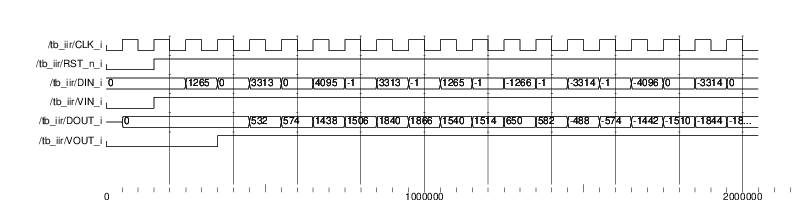
\includegraphics[scale=0.9]{start_sim_post_synth.png}
	\caption{Netlist output after synthesis}
	\label{fig:y_post_synth}
\end{figure}

\newpage
\subsubsection{Place \& Route}
After the synthesis of the filter, place and route operations have been performed with Cadence Innovus,  the clock frequency has been set at f$_{clk}$=$\frac{f_M}{4}$=83,3 MHz, where f$_M$ is the maximum clock frequency when the slack is equals to 0 ns. With this tool, the design of the filter has been imported with the use of \textit{design.globals} and \textit{mmm\_design.tcl} files.\\Then, the cell ensemble area has been assigned by structuring the floorplan and the area of the rings where the power supply routed has been added to this one. %ho controllato la preposizione ed é add to
In particular, the rings are two: one for power supply (V$_{DD}$) and another one for ground (V$_{SS}$).\\Afterwards the horizontal wires of V$_{DD}$ and V$_{SS}$ have been placed for the standard cells. Some of these wires have been connected to the ring as well as to the vertical stripes, thus the cells have been placed.\\
After these steps, the design has been optimized with a \textbf{Post Clock-Tree-Synthesis (CTS) optimization} to achieve the required timing constraints and then the placement has been completed with the use of filler cells that fill the holes to ensure continuity in n+ and p+ wells in each row.\\The last phase has been the routing phase, where the connection among the cells has been performed using the available metal layers. After this one the design has been completed and it has been possible to do another optimization called \textbf{Post routing optimization}, used to achieve the required timing constraints.\\At this point, the layout of the IIR filter reported in Figure \ref{fig:filter_layout} has been created.
 \begin{figure} [h]
\centering
	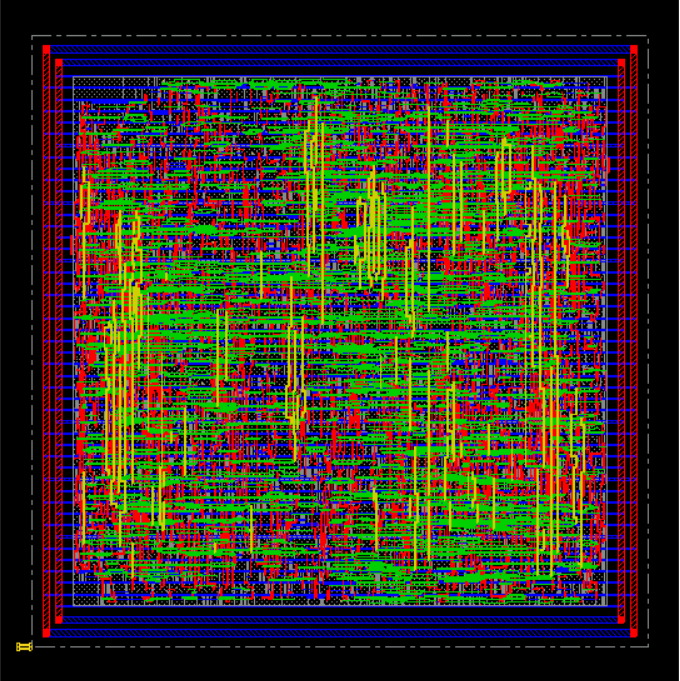
\includegraphics[scale=0.6]{filter_layout.png}
	\caption{IIR filter layout}
	\label{fig:filter_layout}
\end{figure}
\noindent
\newline
Subsequently, an analysis of the time behaviour has been performed taking into account the parasitic resistance and capacitance values for each metal wire.
%resistance and capacitance parasitic value for each metal wire. 
By this analysis, some reports have been produced, one for the \textbf{setup analysis} and another one for the \textbf{hold analysis}. These reports contain general and detailed information on timing paths and violations and in particular about the slack that in both the reports is turned out as positive for every signal and this means that the constraints have been met.\\Afterwards a verification of the connectivity and of the geometry has been done and in each case no violations have been found.\\ At this point it has been possible to extract the value of the area, the gates and the cells of the IIR filter design, that are:
\begin{itemize}
    \item Area= 2497,5 $\mu$m$^2$;
    \item Gates= 3129;
    \item Cells= 1244.
\end{itemize}
Then the last step of the place and route operation has consisted of saving the netlist as a Verilog file in order to use it in the next Simulation step.
\subsubsection{Post place and route simulation and switching-activity-based power consumption estimation}
For this phase Modelsim and Cadence Innovus have been jointly used.\\At the first step the Verilog netlist produced by Innovus and all the test-bench files have been compiled to simulate in Modelsim. The ensuing result %(=il risultato che ne deriva)%
is the switching activity information stored in the \textit{vcd} file named \textit{design.vcd}.\\From the simulation, another output file has been created and this is the \textit{results.txt} which contains the output \textbf{y[n]} of the filter when the used netlist is the one generated by the place and route analysis.\\The values stored in \textit{results.txt}  have been compared with the ones obtained with the VHDL using Matlab, they have turned out to be the same. 
%done the difference between the two output vectors with Matlab. The difference value has resulted in zero and this means that the two output files are equal.
\\Then, for the last step Cadence Innovus has been reused to estimate the power consumption. To carry out that, the timing analysis has been performed another time taking into account the parasitic resistance and capacitance values for each metal wire. After that, a power analysis has been performed using the switching activity information, stored inside the \textit{design.vcd}. The obtained values are reported in Table \ref{tab:tot power}.
\begin{longtable}{*6c}
\caption{Power consumption for post-place \& route base version}
\label{tab:tot power}\\
\toprule
Group & \thead{Internal\\Power [mW]} & \thead{Switching\\Power [mW]} & \thead{Leakage\\Power [mW]} & \thead{Total\\Power  [mW]}& \thead{Percentage\\(\%)}\\
\midrule
\endfirsthead
Group & \thead{Internal\\Power [mW]} & \thead{Switching\\Power [mW]} & \thead{Leakage\\Power [mW]} & \thead{Total\\Power  [mW]}& \thead{Percentage\\(\%)}\\
\midrule
\endhead
\midrule
\endfoot
Sequential & 0,0405 & 0,03076 & 0,003322 & 0,07459 & 6,857 \\
Macro & 0 & 0 & 0 & 0 & 0\\
IO & 0 & 0 & 0 & 0 & 0\\
Combinational & 0,5327 & 0,4329 & 0,04753 & 1,013 & 93,14\\
Clock (Combinational) & 0 & 0 & 0 & 0 & 0\\
Clock (Sequential) & 0 & 0 & 0 & 0 & 0\\
\bottomrule
Total & 0,5732 & 0,4637 & 0,05085 & 1,088 & 100\\
\endlastfoot
\end{longtable}
\noindent
It is possible to observe that the major contribution of power consumption is given by the combinational part (93,14\%), constituted by multipliers and adders, which are the bigger part of the filter. In fact, the sequential part is constituted only by five registers: two at the input of the filter, one in the auto-regressive part of the filter and the last two at the output; and it provides the 6,857\% of the power consumption.

\newpage
\section{Advanced architecture development}
In this section, the goal was to improve the architecture using the \textbf{look-ahead} technique with a degree $J=1$. This procedure leads to a development of  a term in the discrete-time equation, this will be reused in the main equation. This enables a modification of the original DFG making possible the application of the universal techniques (such as retiming and pipelining) inside the feedback loop of the IIR filter, without changing its behaviour even if the look-ahead is a non-universal technique. 
\subsection{Architecture development}
Starting from the original DFG, the look-ahead technique has been applied, replacing the variable \textbf{n} with \textbf{n-1}, one can obtain:
\begin{equation}
    v[n-1]=x[n]-a_{1}v[n-2]
\end{equation}
Using and replacing it in the correct position of the original equation of v[n] , it results as follows:
\begin{equation}
    v[n]=x[n]-a_{1}x[n-1]+a_{1}^2v[n-2]
\end{equation}
From this, one can identify a FIR-like part and an IIR-like part, %then the new equation of v[n] is used in the main one:
the resulting equation of y[n], in which v[n] is used, is the following
\begin{gather}
    y[n]=b_{0}v[n]-b_{1}v[n-1] \\
   %  v[n]=x[n]-a_{1}x[n-1]+a_{1}^2v[n-2]
\end{gather}
As can be seen from the equation, there is a new coefficient $a_{1}^2$, the architecture can be improved if it is possible to calculate this new coefficient in advance without instantiating any additional blocks in the architecture.
Directly mapping the equation in a new DFG which is reported in Figure \ref{fig:dfg_la_filt}, one can identify two FIR-like parts and one IIR-like part with two registers along the loop. 
 \begin{figure} [h]
\centering
	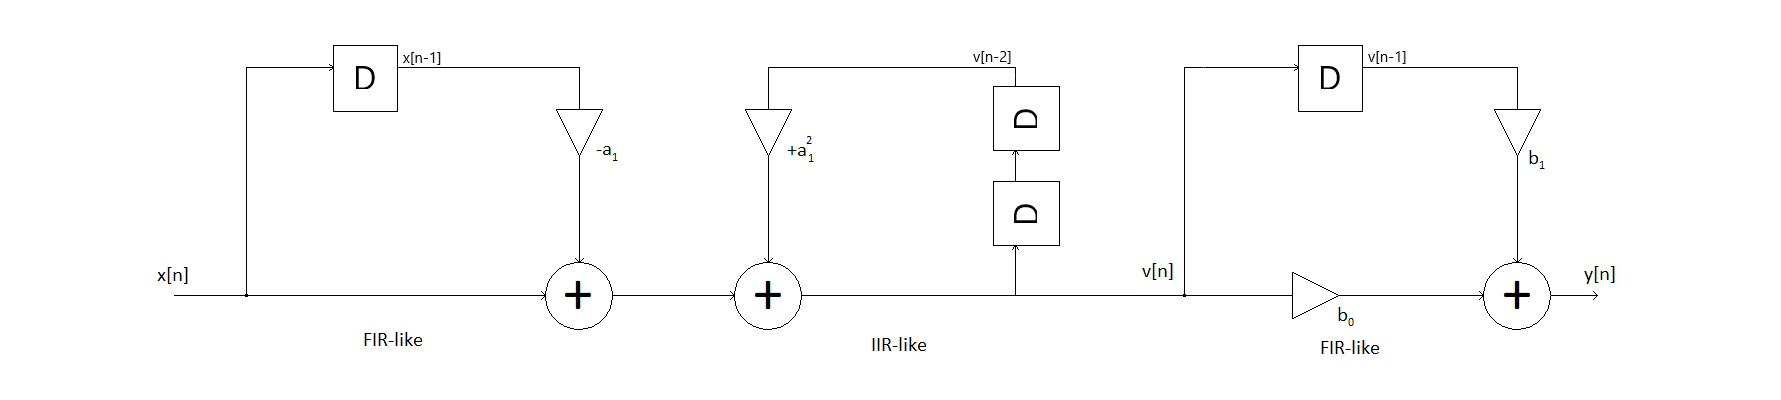
\includegraphics[scale=0.3]{DFG_filter_la.png}
	\caption{"Look-ahead" IIR filter DFG}
	\label{fig:dfg_la_filt}
\end{figure}   
\\
This condition leads to the use of one or more universal technique, for example Retiming or Pipelining. 
\newline In the following figure (Fig. \ref{fig:la_filt}) is shown the new datapath of the filter.

 \begin{figure} [h]
\centering
	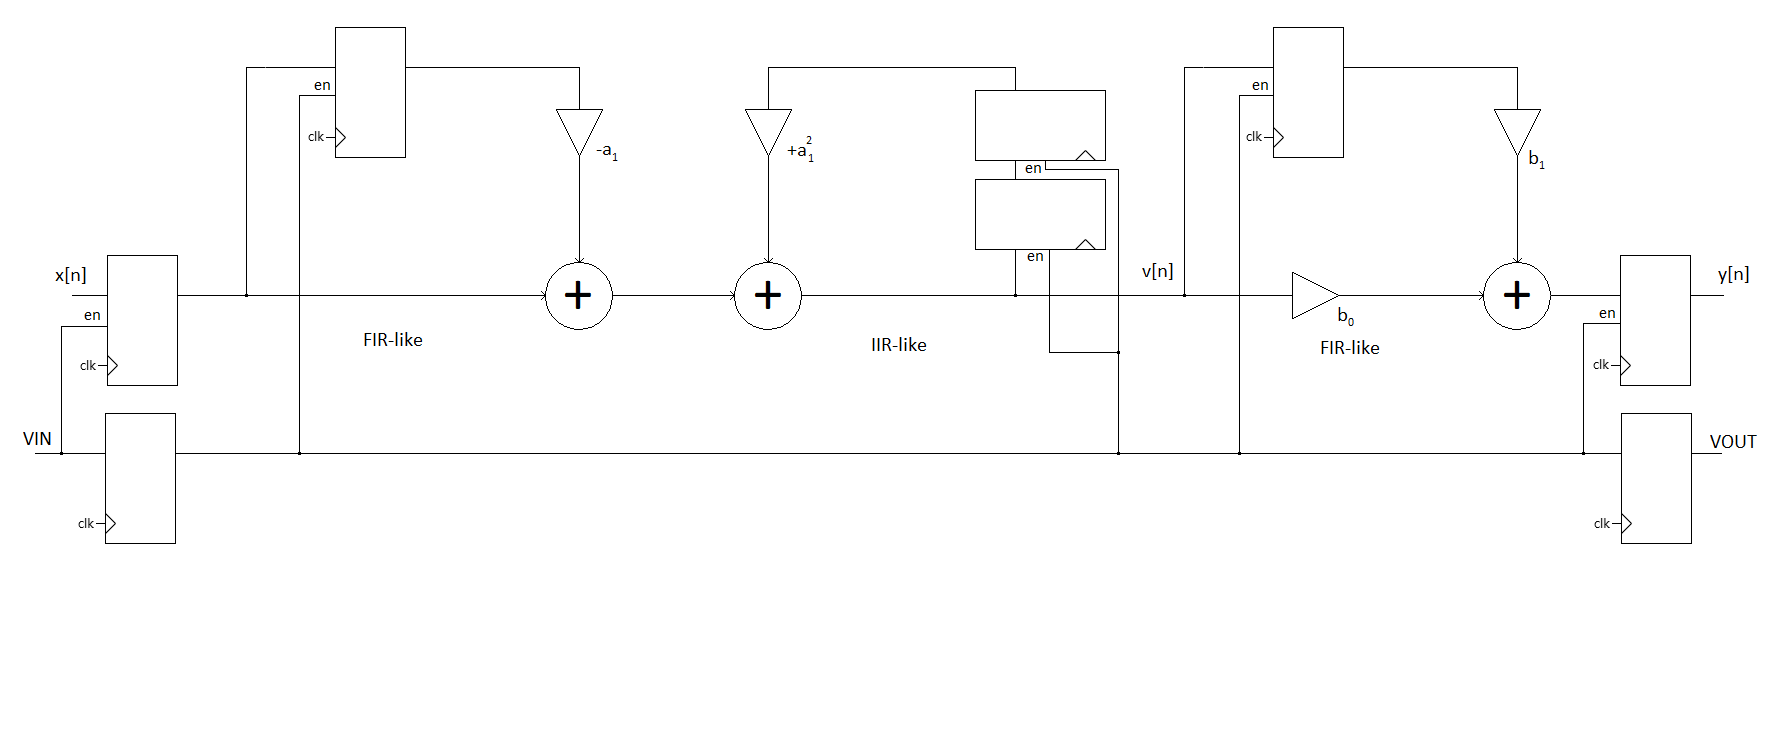
\includegraphics[scale=0.3]{filter_la.png}
	\caption{"Look-ahead" IIR filter datapath}
	\label{fig:la_filt}
\end{figure}
\noindent Also in this case some interface registers are present, driven by VIN, on the contrary this latter signal is sampled in any case and VOUT is generated by properly delaying VIN inside the architecture without adopting any enable signal. The internal registers use as enable the VIN replica.

\noindent
The modified C implementation has been used as a reference to check the constraint on the THD. The base version of the filter implemented in C has been modified according to the new DFG, adopting new variables as registers. The resulting total harmonic distortion is $THD=-74\; dB$, which is less than the original one but the filter has still a good capability to keep low the distortion and it is still satisfying the constraints. In Figure \ref{fig:thd_c_la}
the THD plot of the C filter is reported.

 \begin{figure} [h]
\centering
	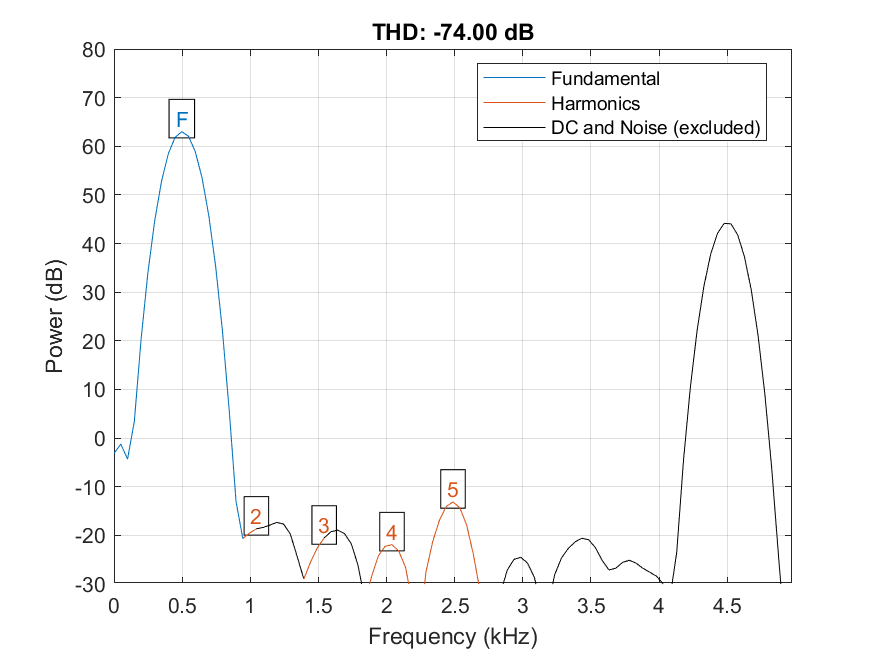
\includegraphics[scale=0.8]{thd_c_la_ref.png}
	\caption{THD "C look-ahead" IIR filter}
	\label{fig:thd_c_la}
\end{figure}
\noindent
The following task of this  section has required to improve the performance of the filter applying several techniques.\\
First of all, $T_{\infty}$ has been calculated, taking into account the only loop present in the filter, which is the one in the IIR-like part, it has resulted:
\begin{equation}
    T_{\infty}=\dfrac{T_a+T_m}{2}
\end{equation}
This value set the achievable value of $T_{cp}$, that without applying any techniques was:
\begin{equation}
    T_{cp}=3 \cdot T_a+2 \cdot T_m
\end{equation}
Since $T_{\infty}$ was less than $T_{cp}$, it has been possible to apply some improvements to the architecture.\\
\textbf{Pipelining} is the first one which has been implemented. With this one, new pipeline registers have been inserted between the FIR-like and the IIR-like parts. In this way the longest path in the circuit has been split, starting from the register before the multiplication by $-a_{1}$ and arriving at the output register. In this first pipeline application two new registers have been used.
\newline
Then, focusing on the first FIR-like part, the \textbf{retiming} technique has been applied. This tries to move the registers in other positions which are equivalent in terms of functions but can lead to a speed improvement reducing the delay of the critical path.\\
In this case, the register before the multiplier by $-a_1$ has been moved after this latter to split the path, starting from the multiplier and arriving at the adder. In this particularly case this approach is preferable to pipelining since implementing this latter technique the implementation cost increases since two additional register are needed (2 additional registers plus the original one vs the original register).
\newline
In the second FIR-like part pipelining has been applied, once a feed-forward cutset has been found between the two multipliers and the adder, two register have been instantiated splitting the two adder-multiplier paths. Obviously this has led to an additional latency of the filter (not counting the other two pipeline stages applied before), but this technique, combined with the others, has drastically improved the speed of the design.\\The DFG related to the application of pipeling and retiming technique is reported in Figure \ref{fig:dfg_la_ret_pp_filt}.
\newpage
 \begin{figure} [h]
\centering
	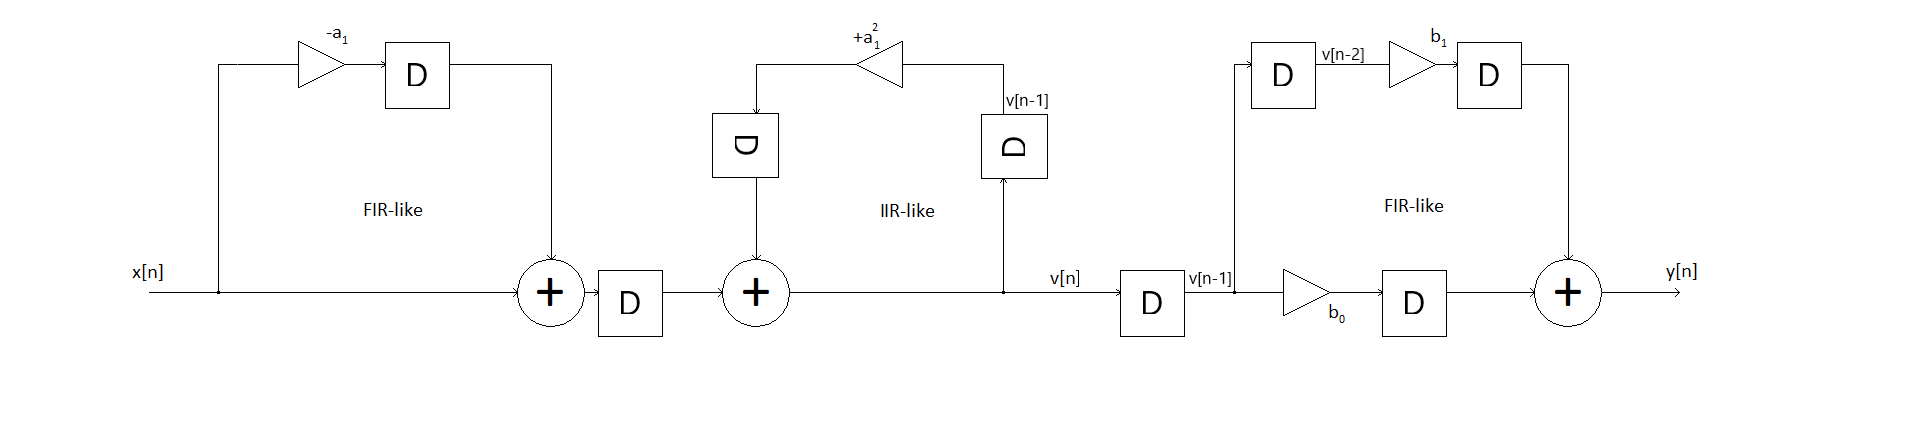
\includegraphics[scale=0.3]{DFG_filter_la_ret_pp.png}
	\caption{Improved "Look-ahead" IIR filter DFG}
	\label{fig:dfg_la_ret_pp_filt}
\end{figure}   
\noindent
At this point the critical path delay has resulted $T_{cp} =max\{T_m,T_a\}$, therefore  the new value of $T_{cp}$ is less than $T_{\infty}$ thus this means that is not possible to furthermore increase the performance of the architecture.
\newline The resulting datapath is shown in the figure below (Fig.\ref{fig:la_filt_ret_pp}).
 \begin{figure} [h]
\centering
	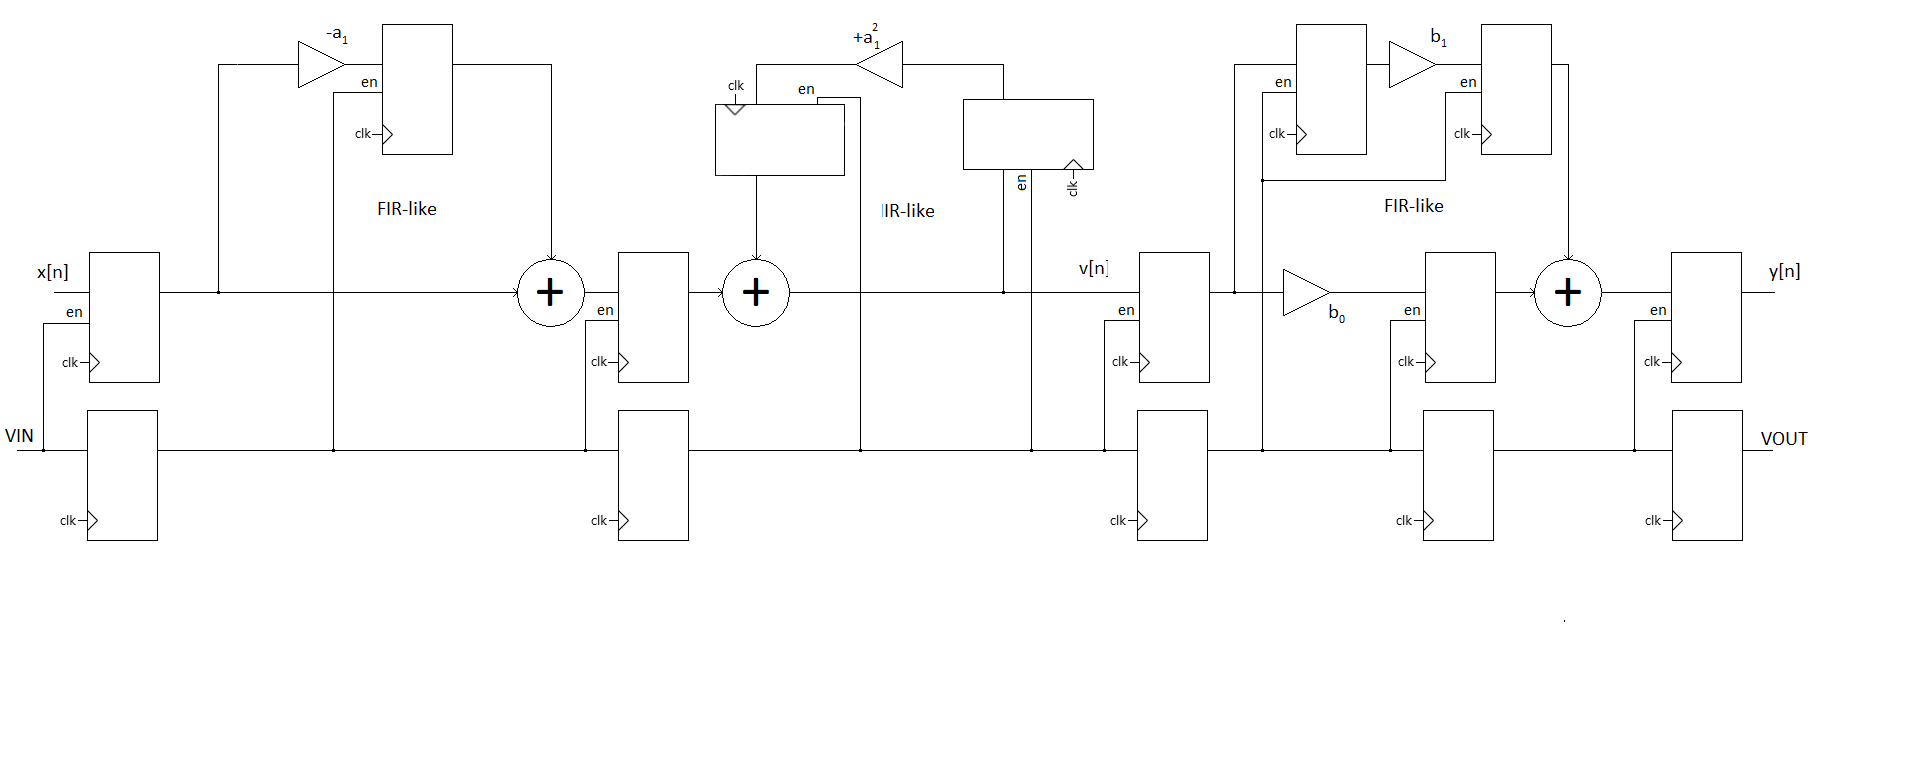
\includegraphics[scale=0.3]{filter_la_ret_pp.png}
	\caption{Improved "look-ahead" IIR filter datapath}
	\label{fig:la_filt_ret_pp}
\end{figure}
\noindent
Since the design implements three internal pipeline registers, VIN has been delayed to drive with the correct timing all the registers of the architecture. The presence of pipeline stages forces to modify the design to synchronise the flowing of data with commands. 
%It is known that also all the command signals have to be delayed to flow in a synchronised way as data. 
For this purpose three additional pipeline registers have been used for the VIN replica. All the other considerations are the same as the previous datapath.
\newline
In theory, the presence of the new coefficient $a_1^2$ could change the bit-width and the precision of the architecture with respect to the starting one. The first assumption has turned to be incorrect, one single additional internal bit has resulted to be enough to avoid the overflow. So the internal parallelism has remained the same as the original one, keeping the internal area as lower as possible without running in overflow during sums and subtractions (all the considerations are similar to the previous case).
Thus in the VHDL implementation, the internal parallelism is equal to 14 bit, a bit-width large enough to ensure all the calculations without computational errors.
%\begin{itemize}
 %   \item Input parallelism = 13 bit (from the specification);
%    \item Internal parallelism = 14 bit.
%%\noindent
The precision has changed, this is probably due to the additional operation in the chain, the new coefficient has been converted in 13 bit fixed point number, this has led to an additional loss of precision in the computation. Also, the additional multiplication and the consequent chopping has contributed to this. This is reasonable, the presence of new coefficients due to the developing of parts of the discrete-time equation, increases the number of operations which have to be implemented in a real hardware system. % with the consequent loss of precision. 
This phenomena is not directly visible in the C implementation, because generally the large number of bits avoid the presence of the overflow, so is not necessary to apply any countermeasure (like the extended internal parallelism ).
\newline
Anyway, the overall THD  of the hardware architecture is still in the constraints and it shows a good attenuation of the unwanted harmonics, which can be observed in the plot reported in fig.\ref{fig:thd_vhdl_la}. It results equal to $THD=-67,06 \; dB$, compared to the reference C (look-ahead version) implementation it has been degraded of only less than $10 \; dB$. Thus, it is possible to notice that the harmonics power has been increased after the modifications applied to the architecture.
 \begin{figure} [h]
\centering
	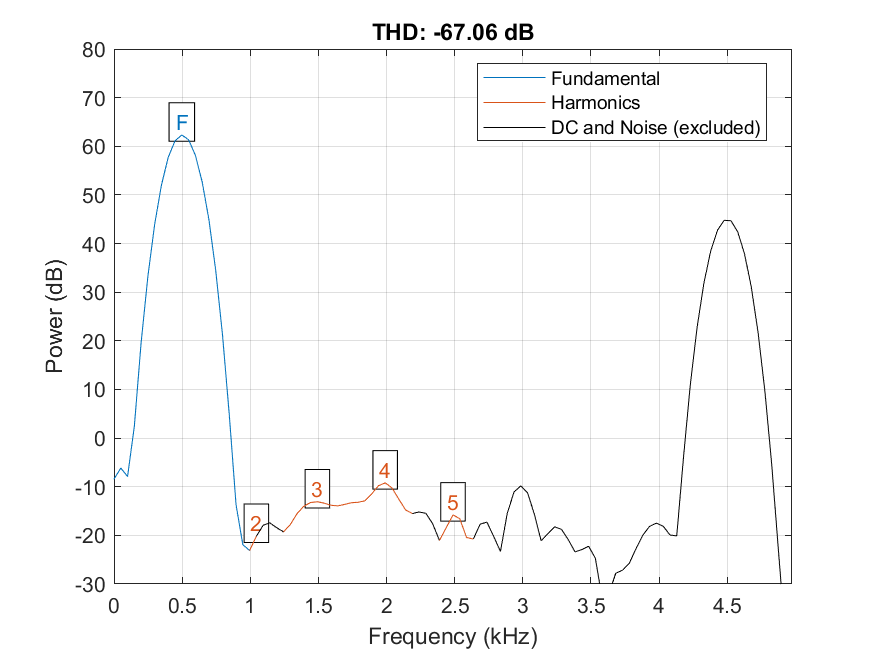
\includegraphics[scale=0.6]{thd_vhdl_la.png}
	\caption{THD "improved look-ahead" IIR filter}
	\label{fig:thd_vhdl_la}
\end{figure}
\newpage
\subsection{Simulation}
The new VHDL design has been simulated with Modelsim and then its results have been compared with the C ones through Matlab performing the difference element by element. Both results has resulted the same and this has confirmed the correctness of the implementation. In Figure \ref{fig:la_start} and Figure \ref{fig:la_vin}, two results of the simulation are reported. In the second one it is possible to notice the correct behaviour of the filter with respect to VIN variations.

 \begin{figure} [h]
\centering
	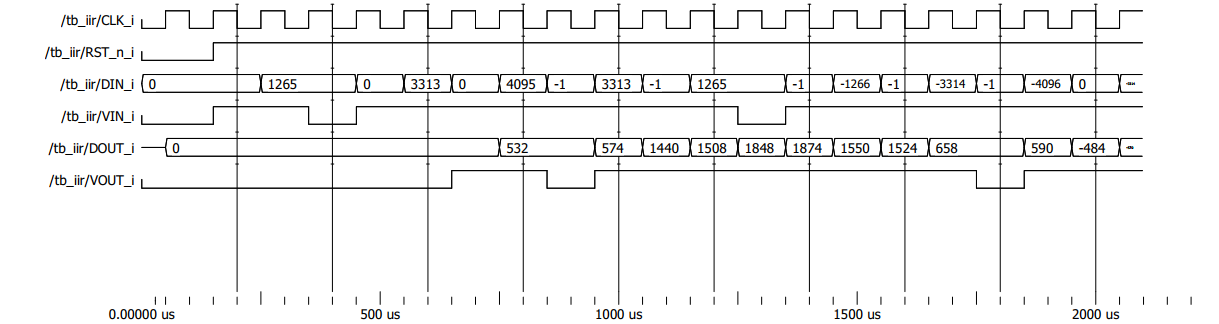
\includegraphics[scale=0.55]{la_vin.png}
	\caption{"Look-ahead" IIR filter simulation}
	\label{fig:la_start}
\end{figure}

 \begin{figure} [h]
\centering
	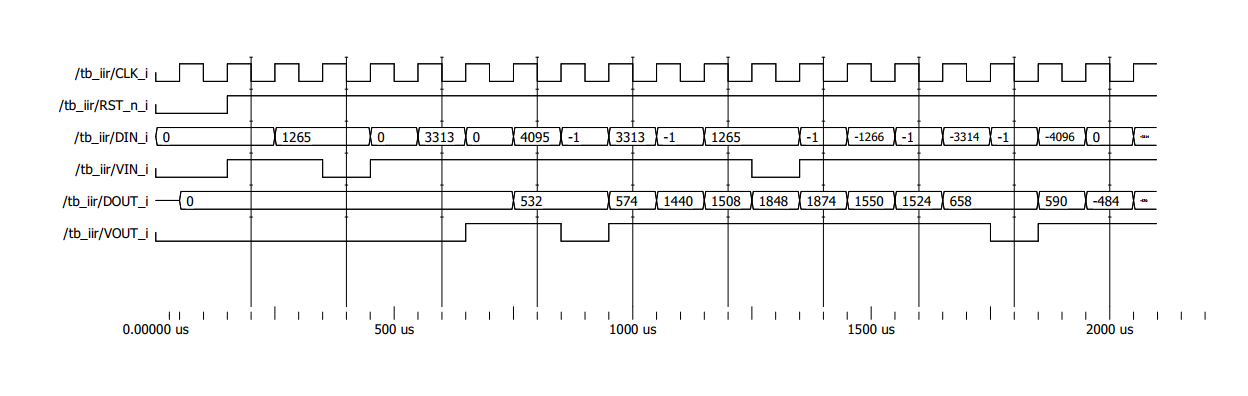
\includegraphics[scale=0.55]{la_start.png}
	\caption{"Look-ahead" IIR filter simulations with VIN variations}
	\label{fig:la_vin}
\end{figure}
\noindent
As one can see from Figure \ref{fig:la_vin}, VIN and DOUT are properly delayed accordingly to the registers present in the design. There are present two interface registers, one at the input and one at the output and three additional registers are allocated inside the architecture due to the pipelining. All these registers introduce a delay equal to five clock cycles, from the simulation it is clear to see that DOUT and VOUT change after exactly 5 clock cycles. This definitely has led to a speed improvement counterbalanced by an additional latency in the filter.
\newpage
\subsection{Implementation}
\subsubsection{Logic synthesis} 
Even for the new architecture the design has been synthesized with Synopsys Design Compiler. In this case $f_M=645,2\;MHz $ (T$_{min}$=1,55 ns) has been obtained as the maximum achievable frequency corresponding to a slack equal to zero.\\Afterward another synthesis has been performed to find the area of the architecture corresponding to $f_M$. Thus the total cell area has resulted equal to $A_{f_M}\simeq4258,13 \; \mu m ^2$. 
\\Then a new synthesis has been performed using a clock frequency $\dfrac{f_M}{4} = 161,3\;MHz$ (T$_{min}$=6,2 ns). In this case the Total Cell Area is $A_{f_M/4}\sim3862,05 \; \mu m ^2$. As in the original version, even in this case the Total Cell Area is decreased and this could depend another time on the instantiation of different elements compared to the case with f$_M$ as clock frequency.\\ Furthermore the Combinational Area and the Buf/inv Area are changed respectively from $\simeq3621,3$ $\mu m^2$ in the case of f$_M$ as clock frequency to $\simeq3229,5$ $\mu m^2$ in the case of $\dfrac{f_M}{4}$ and from $\simeq223,4$ $\mu m^2$ (f$_M$ case) to $\simeq155,6$ $\mu m^2$ ($\dfrac{f_M}{4}$ case) and these decreases are reasonable since the architecture synthesized with $\dfrac{f_M}{4}$ is slower than the one with f$_M$ and requests slower blocks which are less demanding in terms of area. Moreover the minor number of buffer is justified by the fact that the propagation time is longer for the architecture that uses $\dfrac{f_M}{4}$ rather than the architecture with a clock frequency equal to f$_M$, thus the interconnections do not need to be cut with additional buffers.\\
In addiction another observation could be done, %which is that
comparing the Total Cell Area for the original version ($A_{f_M/4}= 2501,46\; \mu m ^2$) and look-ahead version ($A_{f_M/4}= 3862,05\; \mu m ^2$) it is possible to notice an increment of area for the new architecture and this has been due to the addition of registers, adders and multipliers.\\
All these data are reported in Table \ref{tab:area advanced case fm vs fm/4}. 
\begin{longtable}{*6c}
\caption{Area $f_M$ vs Area $\dfrac{f_M}{4}$}
\label{tab:area advanced case fm vs fm/4}\\
\toprule
Clock freq. & \thead{Combinational \;[$\mu m^2$]} & \thead{Buf/Inv\;[$\mu m^2$]} & \thead{Tot.\; Cell \;Area\;[$\mu m^2$]} \\
\midrule
\endfirsthead
Clock freq. & \thead{Combinational \;[$\mu m^2$]} & \thead{Buf/Inv\;[$\mu m^2$]} & \thead{Tot.\; Cell \;Area\;[$\mu m^2$]}  \\
\midrule
\endhead
\midrule
\endfoot
$f_M$ & 3621,3 & 223,4 & 4258,13 \\
$\dfrac{f_M}{4}$ & 3229,5 & 115,6 & 3862,05\\
\bottomrule
\endlastfoot
\end{longtable}
\noindent
Along with period and area, as in the previous synthesis, power reports have been computed, obtaining a total power of $P_{TOT} \simeq 896,13 \; \mu W$ that can be split into different contributions: the power of the combinational part and the power related to the registers which correspond respectively to the value of $\simeq$ 633,39 $\mu$W and $\simeq262,74 \mu$W. These turn out to be higher than the powers on the original version which assume the values of P$_{comb}\simeq$ 272,15 $\mu$W and P$_{reg}\simeq$ 45,97 $\mu$W. The increase of these power is due even in this case to the addition of 10 registers, one adder and one multiplier at the new architecture compared to the original one. As expected, also in this case the Dynamic Power is higher than the Leakage one, all the other considerations are the same as the previous case.
\newpage
\begin{longtable}{*6c} 
\caption{Power consumption for post-synthesis look-ahead version}
\label{tab:power_postsynth_LA}\\
\toprule
Group & \thead{Internal\\Power [$\mu$W]} & \thead{Switching\\Power [$\mu$W]} & \thead{Leakage\\Power [nW]} & \thead{Total\\Power  [$\mu$W]}& \thead{Percentage\\(\%)}\\
\midrule
\endfirsthead
Group & \thead{Internal\\Power [$\mu$W]} & \thead{Switching\\Power [$\mu$W]} & \thead{Leakage\\Power [nW]} & \thead{Total\\Power  [$\mu$W]}& \thead{Percentage\\(\%)}\\
\midrule
\endhead
\midrule
\endfoot
IO pad & 0 & 0 & 0 & 0 & 0\\
Memory & 0 & 0 & 0 & 0 & 0\\
Black box & 0 & 0 & 0 & 0 & 0\\
Clock network & 0 & 0 & 0 & 0 & 0\\
Register & $177,7841$ & $73,9053 $ & $1,1051 \cdot10^{+4}$ & 262,7398 & 29,32\\
Sequential & 0 & 0 & 0 & 0 & 0\\

Combinational  & $326,7868$ & $239,5658$ & $6,7039 \cdot10^{+4}$ & 633,3926 & 70,68\\
\bottomrule
Total & $504,5709$ & $313,4711$ & $7,8090 \cdot10^{+4}$ & 896,1324 & 100\\
\endlastfoot
\end{longtable}
\subsubsection{Place \& route}
The same procedure as in the original architecture has been performed for the look-ahead implementation of the IIR filter with Cadence Innovus.\\In this case the clock frequency which has been used is: f$_{clk}$=$\frac{f_M}{4}$=161,3 MHz, where f$_M$ is the maximum clock frequency when the slack is equal to 0 ns. Thus it is possible to observe that the clock frequency of this optimized version of the filter is increased compared to the original one, therefore the speed has been improved.\\%In these place and route operations 
After place $\&$ route step the layout of the IIR filter has been obtained and it is reported in Figure \ref{fig:filter_layout_LA}.
 \begin{figure} [h]
\centering
	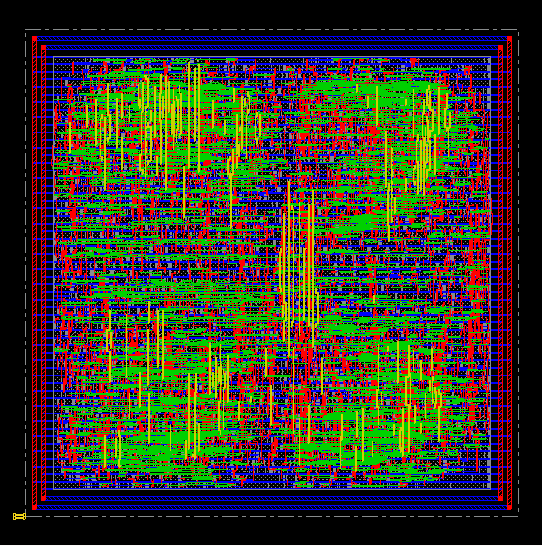
\includegraphics[scale=0.7]{layout_filter_LA.PNG}
	\caption{IIR filter layout of look-ahead version}
	\label{fig:filter_layout_LA}
\end{figure}
\noindent
\newline
Thus comparing this figure with the Figure \ref{fig:filter_layout} related to the original filter, it is possible to notice that the density of the components is increased, in fact in the look-ahead version with pipelining and retiming techniques 10 registers are present instead of 3 as in the original version and the number of adders and multipliers is respectively increased from 2 to 3 and from 3 to 4.\\Even in this case an analysis of the time behavior has been performed taking into account  parasitic resistance and capacitance values for each metal wire and again the slack has resulted positive for each signal, therefore the constraints are met.
\newpage 
\noindent
Moreover for the look-ahead version of the filter the values of the area, gates and cells which have been obtained are:
\begin{itemize}
    \item Area=3842,4 $\mu$m$^2$;
    \item Gates= 4815;
    \item Cells= 1894.
\end{itemize}
Therefore it is possible to observe that the area, the number of gates and cells are increased compared to the original version of the filter as it is reported in Table \ref{tab:comparison area} and this is agreed with the growth of the number of registers, adders and multipliers previously mentioned.\\Then, the netlist has been generated and saved as a Verilog file like before.
\begin{longtable}{*4c}
\caption{Comparison between original version and improved version}
\label{tab:comparison area}\\
\toprule
 & Area [$\mu$m$^2$] & Gates & Cells\\
\midrule
\endfirsthead
 & Area [$\mu$m$^2$] & Gates & Cells\\
\midrule
\endhead
\midrule
\endfoot
original version & 2497,5 & 3129 & 1244 \\
improved version & 3842,4 & 4815 & 1894\\
\bottomrule
\endlastfoot
\end{longtable}
\subsubsection{Post place and route simulation and switching-activity-based power consumption estimation}
Similarly to the previous case, the Verilog netlist produced by Innovus and all the test-bench files have been compiled to simulate in Modelsim. Thus by this simulation 2 files have been generated: \textit{design.vcd}, which will be used for the analysis of the power consumption, and \textit{results.txt}, that contains the output of the filter generated by the simulation.\\ The last one has been compared again with the output results of the base VHDL version (without the look-ahead implementation), but in this case, the difference between these two outputs doesn't give zero because in the look-ahead version is present a new coefficient \textit{a$_1${$^2$}} which has been computed and quantized in Matlab and this involves in a quantization error in addition to the rounding errors introduced in the new operation.
\\ Anyway the results of the VHDL version and the modified C version (look-ahead like) are the same, this ensures the correctness of the hardware implementation.
\\Then, the power analysis has been performed another time even for the optimized version of the IIR filter using the information about the switching activities inside the \textit{design.vcd} file. The obtained values are reported in Table \ref{tab:tot power LA}.
\begin{longtable}{*6c}
\caption{Power consumption for look-ahead version}
\label{tab:tot power LA}\\
\toprule
Group & \thead{Internal\\Power [mW]} & \thead{Switching\\Power [mW]} & \thead{Leakage\\Power [mW]} & \thead{Total\\Power  [mW]}& \thead{Percentage\\(\%)}\\
\midrule
\endfirsthead
Group & \thead{Internal\\Power [mW]} & \thead{Switching\\Power [mW]} & \thead{Leakage\\Power [mW]} & \thead{Total\\Power  [mW]}& \thead{Percentage\\(\%)}\\
\midrule
\endhead
\midrule
\endfoot
Sequential & 0,2663 & 0,1071 & 0,01097 & 0,3843 & 21,19 \\
Macro & 0 & 0 & 0 & 0 & 0\\
IO & 0 & 0 & 0 & 0 & 0\\
Combinational & 0,7746 & 0,5877 & 0,06681 & 1,429 & 78,81\\
Clock (Combinational) & 0 & 0 & 0 & 0 & 0\\
Clock (Sequential) & 0 & 0 & 0 & 0 & 0\\
\bottomrule
Total & 1,041 & 0,6948 & 0,07777 & 1,813 & 100\\
\endlastfoot
\end{longtable}
\noindent
In this case the contribution of the sequential part is increased from 0,07459$\;\mu$W of the original version to 0,3843 mW of the look-ahead version and it is again caused by the growth of the quantity of registers. Moreover the power consumption of the combinational part is increased, in fact the total power for the look-ahead version is 1,429 mW while in the original version was 1,013 mW and this is due to the presence of an extra multiplier and an extra adder.
\newpage
\subsection{Comparison between synthesys power and place \& route power}
After finishing all the power analysis both for synthesys and for place and route, these have been compared each other and the value which has been obtained by the ratio between the place and route total power and the synthesys total power is approximately three:
\begin{equation}
    \dfrac{Place\; and\; route\;  Tot. \;power}{Syntesys\; Tot. \;power} \simeq 3
\end{equation}
This value is valid both for the case of the original version of the IIR filter and for the optimization version where the look-ahead, pipelining and retiming techiniques have been adopted.\\The fact that the synthesys power is less than the place and route power happens because Synopsys could not manage to take into account all the real power contributions since the library that it considers is an academic library.
\newline
In Table \ref{tab:comparison} and Table \ref{tab:synth_placeroute_power_la} are reported, respectively for the base version case and the final improved case, all the values of power related to the Synthesis and Place \& Route steps, it is shown also the ratio between both Total Power and all the percentage increases of different components of power.
\newline
It is important to notice that the ratio in the improved architecture is roughly 2, but this is reasonable because in this specific the ratio equal to  3 is only a rule of thumb and it is not a constraint. 
\begin{longtable}{*5c}
\caption{Synthesys Power vs Place \& Route power for original version architecture}
\label{tab:comparison}\\
\toprule
Step &  \thead{Internal\\Power [$\mu$W]} &  \thead{Switching\\Power [$\mu$W]} &  \thead{Leakage\\Power [nW]} &  \thead{Total\\Power [$\mu$W]}\\
\midrule
\endfirsthead
Step &  \thead{Internal\\Power [$\mu$W]} &  \thead{Switching\\Power [$\mu$W]} &  \thead{Leakage\\Power [nW]} &  \thead{Total\\Power [$\mu$W]}\\
\midrule
\endhead
\midrule
\endfoot
Synthesys & 157,8943 & 109,7192 & $5,0508\cdot 10^4$ & 318,1216  \\
Place \& Route & 573,2031 & 463,6733 & $5,0847\cdot 10^4$ & 1087,724\\
\bottomrule
Inc.\% & 263,023 & 322,6 & 0,672  & 248,493 \\
Ratio & / & / & / & 3,48 \\
\bottomrule
\endlastfoot
\end{longtable}

\begin{longtable}{*5c}
\caption{Synthesys Power vs Place \& Route power for improved version architecture}
\label{tab:synth_placeroute_power_la}\\
\toprule
Step &  \thead{Internal\\Power [$\mu$W]} &  \thead{Switching\\Power [$\mu$W]} &  \thead{Leakage\\Power [nW]} &  \thead{Total\\Power [$\mu$W]}\\
\midrule
\endfirsthead
Step &  \thead{Internal\\Power [$\mu$W]} &  \thead{Switching\\Power [$\mu$W]} &  \thead{Leakage\\Power [nW]} &  \thead{Total\\Power [$\mu$W]}\\
\midrule
\endhead
\midrule
\endfoot
Synthesys & 504,5709 & 313,4711 & $7,8090\cdot 10^4$ & 896,1324  \\
Place \& Route & 1040,86 & 694,7629 & $7,7774 \cdot 10^4$ & 1813,397\\
\bottomrule
Inc.\%& 106,286 & 121,635 & -0,404  & 102,358 \\
Ratio & / & / & / & 2,024 \\
\bottomrule
\endlastfoot
\end{longtable}
\end{document}
  
